\documentclass{beamer}
\usepackage[utf8]{inputenc}
\uselanguage{French}
\languagepath{French}
\usepackage{utopia} %font utopia imported

\newcommand{\figref}[1]{\figurename~\ref{#1}}
\usetheme{Default}
\usecolortheme{seahorse}
\setbeamertemplate{caption}[numbered]

\usepackage{scalerel}
%------------------------------------------------------------
%This block of code defines the information to appear in the
%Title page
\title[Mode d'utlisation SVN] %optional
{Mode d'utilisation de Subversion SVN pour la RC et Qualité}

\author[HOUEKPETODJI, Honoré] % (optional)
{ H.~Honoré}
\date [2019] % (optional)
{CIM 2019}

\logo{
\includegraphics[height=1.5cm]{../images/logo-cim.jpg}}

%End of title page configuration block
%------------------------------------------------------------



%------------------------------------------------------------
%The next block of commands puts the table of contents at the 
%beginning of each section and highlights the current section:

\AtBeginSection[]
{
  \begin{frame}
    \frametitle{Plan}
    \tableofcontents[currentsection]
  \end{frame}
}
%------------------------------------------------------------


\begin{document}

%The next statement creates the title page.
\frame{\titlepage}


%---------------------------------------------------------
%This block of code is for the table of contents after
%the title page
\begin{frame}
\frametitle{Plan}
\tableofcontents
\end{frame}
%---------------------------------------------------------

\section{SVN}
\begin{frame}
\frametitle{SVN}
\begin{block}{SVN}
SVN est un outil de contrôle de version. SVN est utilisé pour améliorer le travail collaboratif des développeurs sur Izy Protect.
\end{block}

\end{frame}

\section{Préparation de l'environnement de travail}

%---------------------------------------------------------
%Changing visivility of the text
\begin{frame}[label={preparation}]
\frametitle{Pré-requis}
Les pré-requis pour suivre ce manuel sont:
\begin{itemize}
    \item Système d'exploitation Windows
    \item \alert{URL} du projet fournit par le Manager de l'équipe de développement
\end{itemize}
\end{frame}

\begin{frame}
\frametitle{Installation d'outil complémentaire: TortoiseSVN }
\begin{itemize}
\item Aller sur le site de téléchargement de \href{https://tortoisesvn.net/downloads.html}{\beamergotobutton{TortoiseSVN}}. 
\end{itemize}
\end{frame}
%---------------------------------------------------- debut Imprimer ecran du site de telechargement de svn

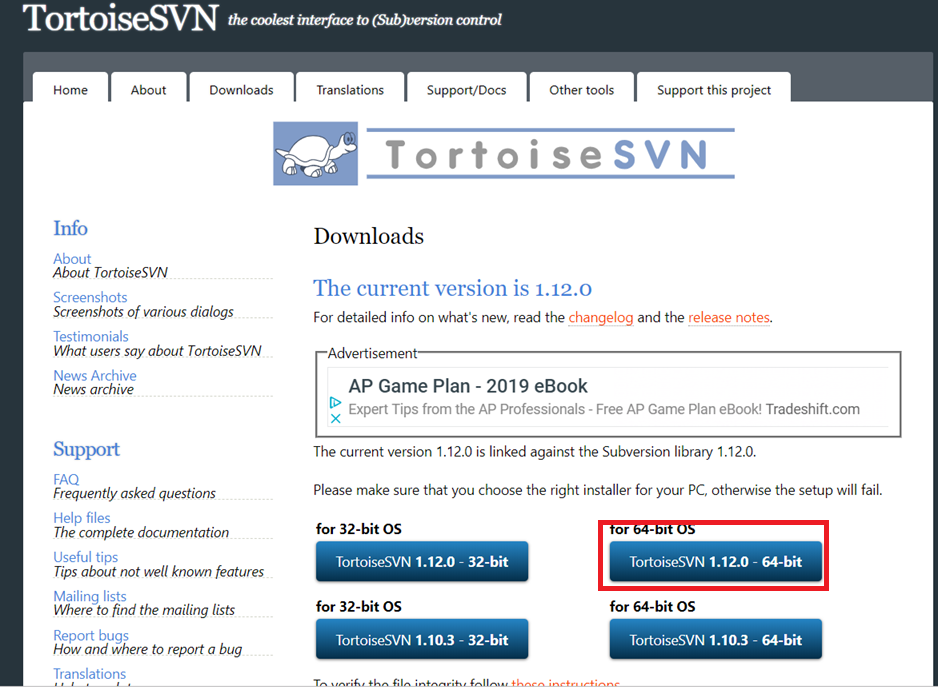
\includegraphics[width=0.9\textwidth]{../images/tortoisesvnDownload.png}
%---------------------------------------------------- fin Imprimer ecran du site de telechargement de svn
\begin{frame}
\frametitle{Installation d'outil complémentaire: TortoiseSVN }
\begin{itemize}
\item Télécharger un installateur en fonction de votre version de Windows( TortoiseSVN 1.12.0 -64-bit) 
\item Aller dans votre dossier de téléchargement Windows 
\item Double cliquer sur l'installateur
\end{itemize}
\end{frame}

\begin{frame}
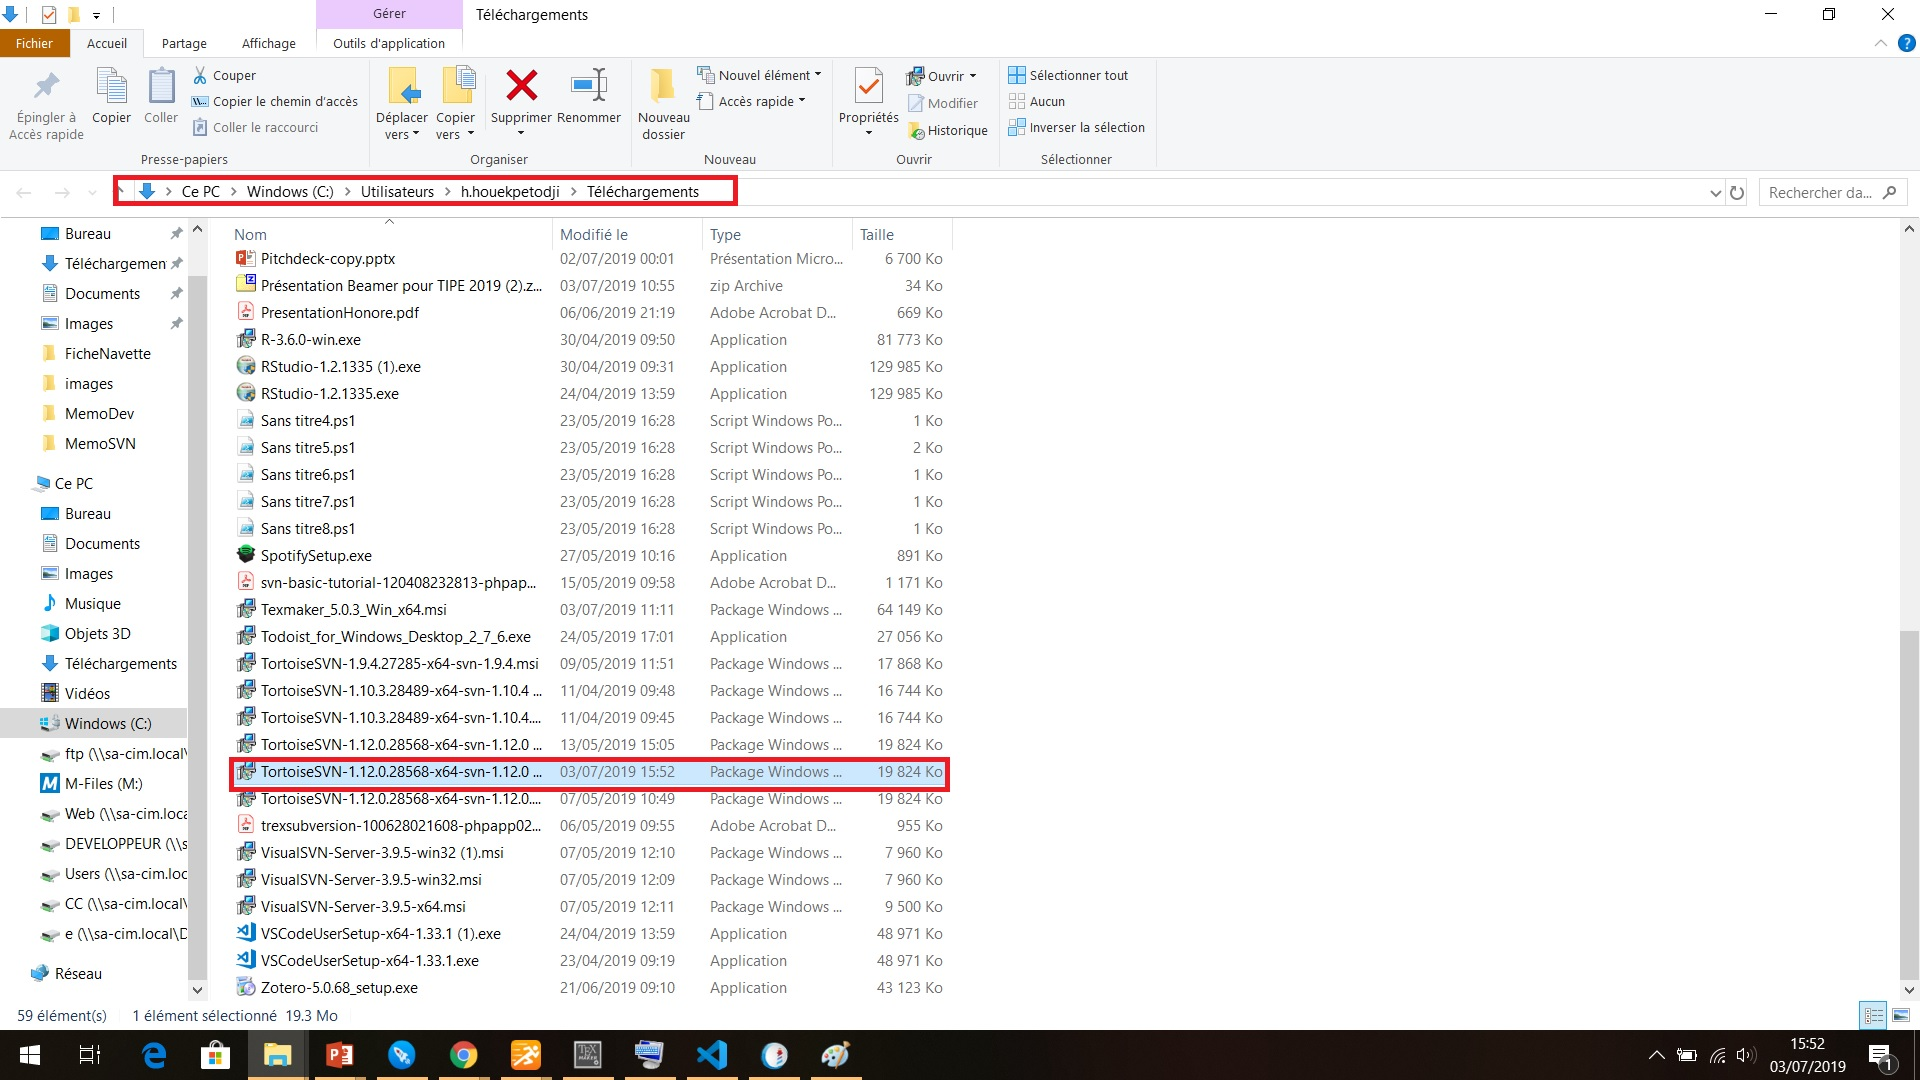
\includegraphics[width=\textwidth]{../images/tortoiseSvnDownloded.jpg}
\end{frame}

\begin{frame}
\frametitle{Installation d'outil complémentaire: TortoiseSVN}
  \begin{columns}[T]
    \begin{column}{.4\textwidth}
     \begin{block}{Étape 1}
Cliquer sur le Bouton \alert{Next}
    \end{block}
     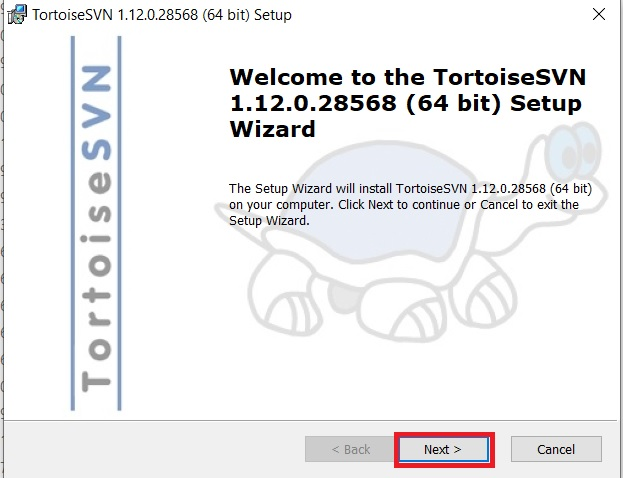
\includegraphics[width=\textwidth]{../images/intalstp1.jpg}
    \end{column}
    \begin{column}{.4\textwidth}
     \begin{block}{Étape 2}
Cliquer sur le Bouton \alert{Next}
    \end{block}
     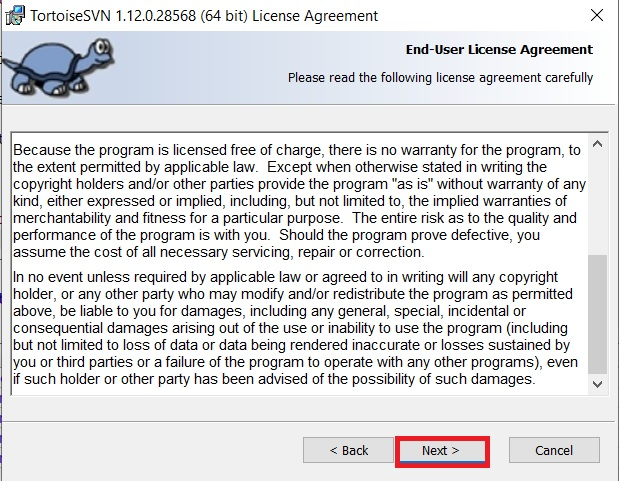
\includegraphics[width=\textwidth]{../images/intalstp2.jpg}
    \end{column}
  \end{columns}
\end{frame}

\begin{frame}
\frametitle{Installation d'outil complémentaire: TortoiseSVN}
  \begin{columns}[T]
    \begin{column}{.4\textwidth}
     \begin{block}{Étape 3}
Cliquer sur le Bouton \alert{Next}
    \end{block}
     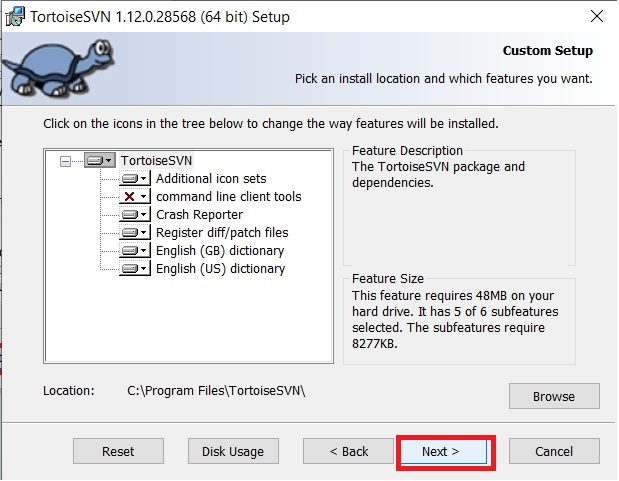
\includegraphics[width=\textwidth]{../images/intalstp3.jpg}
    \end{column}
    \begin{column}{.4\textwidth}
     \begin{block}{Étape 4}
Cliquer sur le Bouton \alert{Next}
    \end{block}
     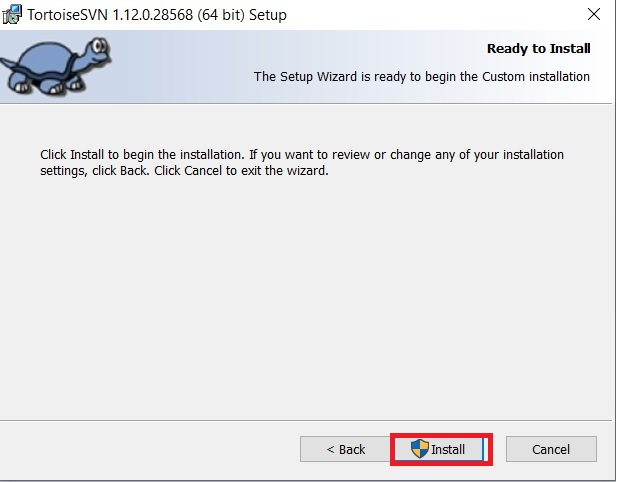
\includegraphics[width=\textwidth]{../images/intalstp4.jpg}
    \end{column}
  \end{columns}
\end{frame}

\section{Utilisation de SVN avec TortoiseSVN}

\begin{frame}
\frametitle{Utilisation de TortoiseSVN}
Dans cette partie, nous supposons que TortoiseSVN a été  installé sur votre machine. Si ce n'est pas le cas, veuillez suivre le slide ~\ref{preparation}.
\end{frame}

\begin{frame}
\frametitle{Utilisation de TortoiseSVN}
\begin{block}{Récupérer un projet depuis le dépôt SVN }
L'action de récupération de projet depuis le dépôt SVN est appelé :  \alert{\textit{Checkout}}. Avec TortoiseSVN, il faut disposer de l'URL vers le projet dans le dépôt SVN. L'URL est fournit par le manager du projet. De plus il faut un dossier vide dans lequel TortoiseSVN va mettre le projet.  Ensuite, il faut
\begin{itemize}
\item Cliquer droit n'importe où dans Windows et choisir l'option \alert{\textit{SVN Checkout}}.
\end{itemize}
\end{block}
\end{frame}
\begin{frame}
\frametitle{Utilisation de TortoiseSVN}
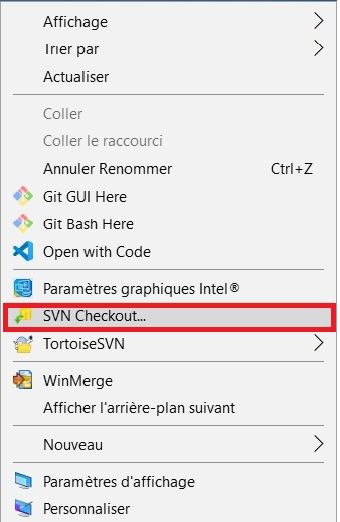
\includegraphics[scale=0.25]{../images/checkout1.jpg}
\begin{block}{Récupérer un projet }

\begin{itemize}
\item Spécifier respectivement, l'URL du projet et le dossier destination
\end{itemize}
\end{block}
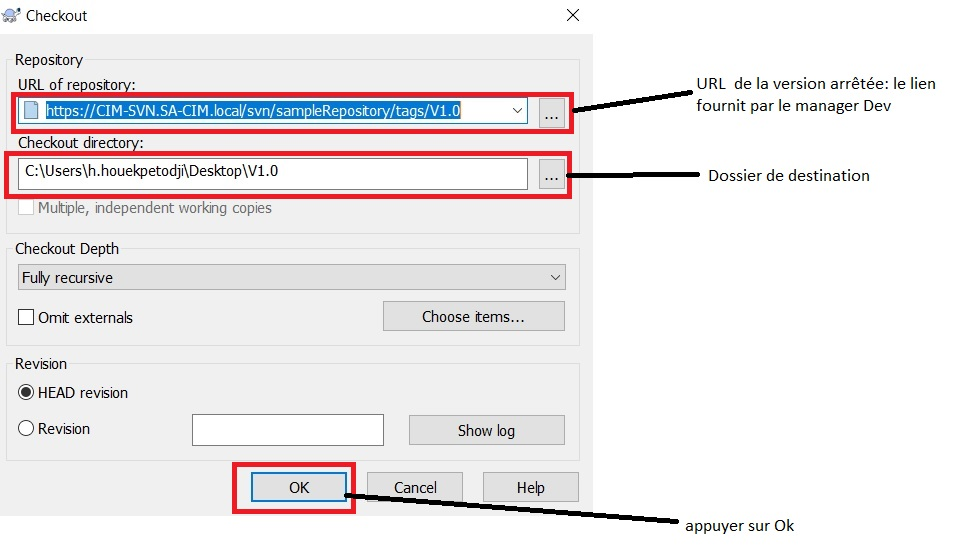
\includegraphics[scale=0.25]{../images/checkout3RC.jpg}
\end{frame}

\begin{frame}
\frametitle{Utilisation de TortoiseSVN}
\begin{block}{Récupérer un projet }
\begin{itemize}
\item Patienter un peu
\item Cliquer sur ok
\end{itemize}
\end{block}
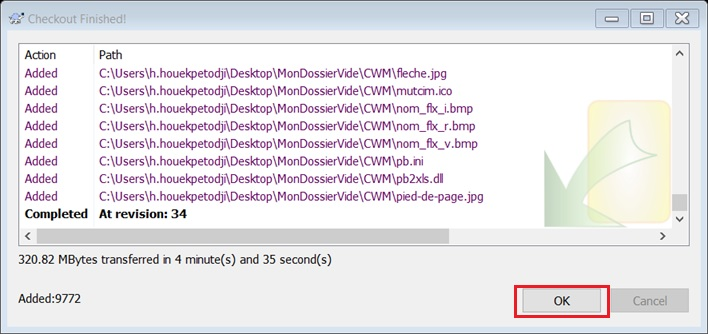
\includegraphics[scale=0.3]{../images/checkout3.jpg}
\newline
\newline
\newline
Finalement le dossier initialement vide contient le projet.
\end{frame}

\begin{frame}
\frametitle{Utilisation de TortoiseSVN}
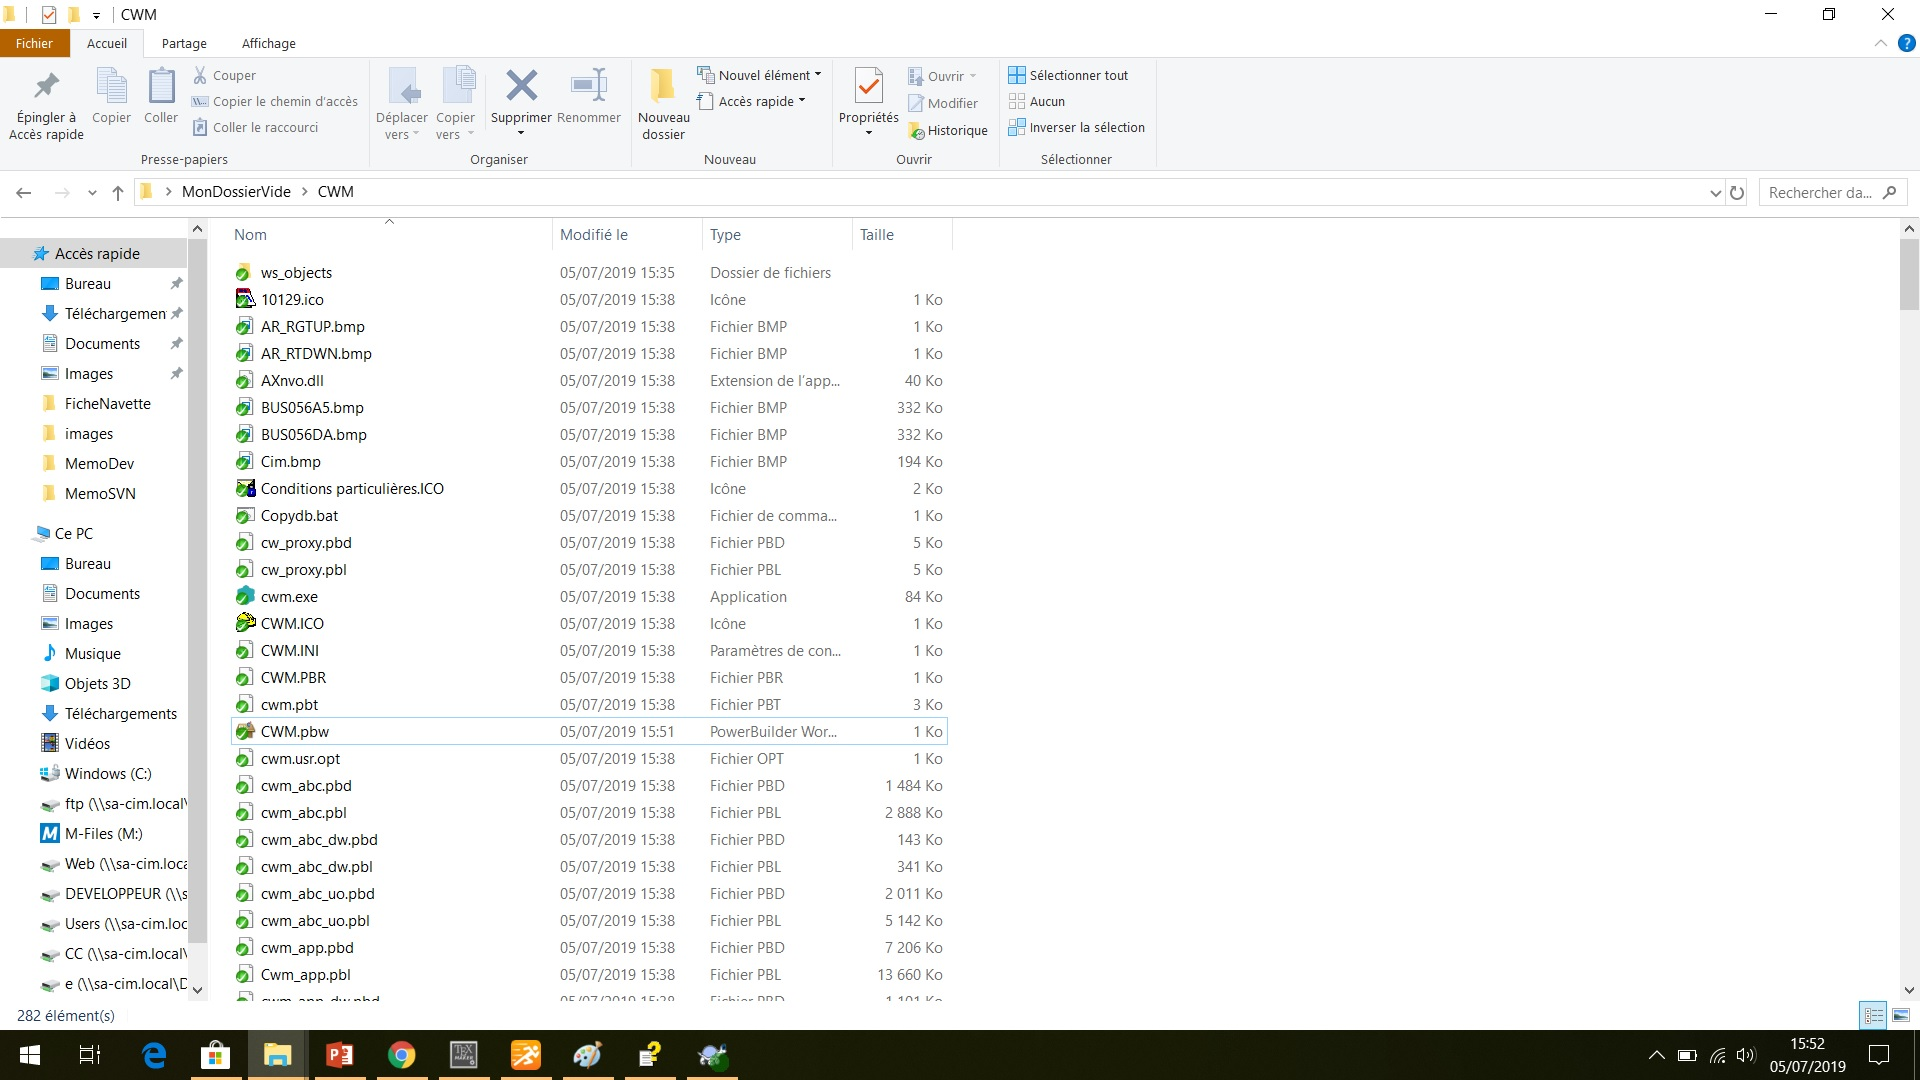
\includegraphics[scale=0.25]{../images/checkout4.jpg}
\end{frame}
\end{document}